%--------------------
% Packages
% -------------------
\documentclass[12pt,english,letterpaper]{article}
\usepackage[T1]{fontenc}
%\usepackage{gentium}
\usepackage{mathptmx} % Use Times Font

\usepackage[utf8]{inputenc}
\usepackage{babel,csquotes,xpatch}% recommended
\usepackage[backend=biber,<options>]{biblatex}

\usepackage[pdftex]{graphicx} % Required for including pictures
\usepackage[pdftex,linkcolor=black,pdfborder={0 0 0}]{hyperref} % Format links for pdf
\usepackage{calc} % To reset the counter in the document after title page
\usepackage{enumitem} % Includes lists

\usepackage[all]{nowidow} % Tries to remove widows
\usepackage[protrusion=true,expansion=true]{microtype} % Improves typography, load after fontpackage is selected

\usepackage{matlab-prettifier}

\usepackage{amsmath}

\addbibresource{sources.bib}

%-----------------------
\hypersetup{ 	
pdftitle = {Classification and Regression Trees},
pdfauthor = {Grant McNaughton}
}

\title{Classification and Regression Trees}
\author{Grant McNaughton}
\date{December 2023}

%-----------------------
% Begin document
%-----------------------
\begin{document} 
\maketitle

\section{Introduction}

Decision trees have long been used as an easy way to guide decision making in a simple and visually clear way. Some of the earliest known decision trees date to the 12th and 13th centuries, and they became an especially popular tool in the medical field starting in the 18th century \cite{lima}. Even today, they are still often used in medical diagnostics guides in combination with other logical operators as a standard means of diagnosis and prognosis.

The first forms of what could reasonably be considered a statistical decision tree first appeared in the 1960s as a natural extension of applying graphs to computer science. References to trees in computer algorithm development can be found as early as 1961 \cite{feigenbaum}, and texts directly discussing the subject can be found as early as 1962 \cite{quinlan}. Despite these early papers, decision tree learning only came to be considered a viable method of large-scale statistical analysis with Breiman et al.’s \textit{Classification and Regression Trees}, published in 1984.\cite{breiman}

Working from Stanford University and the University of California, Berkeley, Breiman et al. developed a fully fleshed and rigorous method for creating useful trees with minimal error. This has since become the foundational text of many related methods, and is still a regularly cited resource today. Breiman et al. first develop a method for creating classification trees, then use those ideas to expand into creating regression trees. They also provided a full analysis of known strengths and weaknesses of the method and provided a set of possible applications at a level not reached previously.

Since then, decision trees have become a standard feature in machine learning software and algorithm design. Essentially every major coding language and platform includes both a classification tree function and a regression tree function, and they present the unique advantage of their inherently visual nature for data visualization.

\section{Foundational Ideas}

The basic idea of CART is to examine all possible splits in the data and determine which split creates the most significant difference between the resulting sets. It does this repeatedly starting from the root node of the tree and can theoretically be repeated until all data points are in a unique terminal node, although it is generally considered best practice to try to keep nodes at a minimum of 5 data points. These large trees can then be “pruned” and combined into more practically applicable forms.

\subsection*{Impurity Metrics}
"Impurity" can take on the form of a few different metrics, but the ones most commonly used are misclassification rate, the Gini measure of dispersion (or Gini metric), and entropy impurity. Breiman et al. developed all of these metrics with regard to CART, which provide progressively smoother impurity functions than the one listed previously.

The misclassification impurity is defined as
\[
i(\tau)=1-maxP(c_j)
\]
with $P(c_j)$ representing the probability of the case in the node being examined. By examining how many cases would be misclassified if we were to use only the mode of the node, we create a linear relationship between the cases and our impurity measure. Misclassification impurity is the simplest form of impurity and is the least commonly used of the three methods, as it often suffers from its simple nature \cite{ma}.

The Gini measure of dispersion is defined as 
\[
i(\tau)=1-\sum_{j=1}^n P (c_j)^2
\]
Because of its quadratic nature, it creates a smoother curve and can be calculated quickly compared to the entropy impurity.

The entropy impurity is defined as
\[i(\tau)=-\sum_{j=1}^n P(c_j)\text{log}P(c_j)\]
This is the most commonly used measure and is the default in many decision tree algorithms. It takes a bit longer to compute but has a strong basis in information theory \cite{duda} and yields the smoothest distribution curve.

\subsection*{Tree growth}
The first step in decision tree learning is growing the tree from a root node. The root node consists of the entire data set and should have the highest impurity of any node in the tree. We then consider all possible splits on the independent variables and assign them a degree of reduction in impurity defined as
\[
\Delta i=i(\tau)-i(\tau_L) \frac{n_1}{n_1+n_2}-i(\tau_R) \frac{n_2}{n_1+n_2}
\]
where $\tau_L$ and $\tau_R$ are the right and left child nodes and the fractions represent the probability of a case being assigned to a child node. This scaling based on probability is important to prevent the algorithm from simply partitioning off very small groups until many terminal nodes are found.

As previously stated, the decision tree could theoretically be partitioned until every node is the smallest size possible, but this will overfit the data to a high degree and make our tree perform poorly when applied to new data. To prevent this, algorithms use chi-squared and a cost-complexity measure developed by Breiman et al. The cost-complexity measure is defined as
\[R_\alpha(T)=R(T)+\alpha|T|\]
where $R(T)$ is the impurity of the node or tree, $|T|$ is the number of nodes in the tree, and $\alpha$ is a chosen penalty coefficient. For this measure, larger values of $\alpha$ correspond to smaller, simpler trees. Using this complexity-weighted impurity in conjunction with a minimum allowable impurity can create trees with strongly defined nodes that end on their own accord.

Another alternative to limiting tree growth is the chi-square statistic, defined in this case as
\[
\chi ^2=\frac{(n_{1L}-Pn_1)^2}{Pn_1}-\frac{(n_{2L}-Pn_2)^2}{Pn_2}
\]
This is used to compare the partition with a random partition, then compared with a critical value $\alpha$, which is determined by degrees of freedom and sample size. If the chi-square is less than $\alpha$, the split does not occur. While stopping tree growth preemptively can be an effective way to avoid overfitting data, a more common approach is to use pruning.

\subsection*{Pruning}
A common alternative to stopping the growth of the tree is to let the tree grow to its maximal size then remove, or "prune," any statistically insignificant nodes. This attempts to minimize the horizon effect as best as possible, but can be much more computationally costly \cite{duda}. Pruning always starts from the terminal nodes and is repeated until the tree is sufficiently simplified.

One of the most common methods for pruning trees is the one standard error rule, which works by defining a standard error determined by risk and sample size
\[SE=\sqrt{\frac{R(T)(1-R(T))}{N}}\]
The risk of the maximal tree is then summed with the standard error to determine the maximum allowable risk of the final tree. All possible trees within the maximal tree are then examined and the largest tree with low enough risk is chosen to be the final tree. \cite{ma}

Any useful tree should be either stopped preemptively or pruned in some way to avoid overfitting the data. Pruning is particularly advantageous when combined with cost-complexity measures, as using cost-complexity while growing the tree tends to force unstable development that does not work well in conjunction with other methods.

\subsection*{MATLAB's Interpretation}
When aggregated together, the algorithm to develop a classification tree is fairly simple. I have chosen to discuss MATLAB's implementation of the concepts because of its popularity in institutional uses and because it was used to find the tree developed on the dummy data below. \cite{matlab}

First, the weighted impurity of each node is defined (using Gini index as the default measure of impurity). Next, the probability of each node is defined as $P(T)=\sum_{j\in T} w_j$ for weight $w_j$ . By default, $w_j=\frac{1}{n}$ and $P(T)=\frac{\text{Size}(T)}{n}$. MATLAB then examines every possible split in the data, piecewise by variable and entry, and determines which split within each category would be the best. Finally, MATLAB determines which split will maximize the impurity gain defined as $\Delta I=P(T)i_t - P(T_L)i_{t_L} - P(T_R)i_{t_R}$.  Altogether, this algorithm can be written as
$$
\max \Delta I = \frac{1}{n} ({\text{Size}(T)}(1-\sum_i p^2(i)) - {\text{Size}(T_L)}(1-\sum_{i_L} p^2(i_L)) - {\text{Size}(T_R)}(1-\sum_{i_R} p^2(i_R)))
$$
MATLAB will continue this process until either reaches a preset limit (maximum number of splits, minimum parent node size with default 10 observations, or minimum leaf node size with default 1 observation), no possible split will yield a positive $\Delta I$, or a node is pure. MATLAB is also capable of using curvature tests to stop tree growth, but it is often preferable to simply let the tree grow completely and prune afterward.

This formulation of CART is less computationally costly than others, as it is very straightforward and does not use any risk measure. The hyperparameters can be easily changed to produce a more or less fitting tree, or can be altogether replaced with a variety of other options to best suit the needs of the data.

\section{Example on dummy data set}

This section concerns the data set "Cereal," (attached) and includes the manufacturer and nutrition information per cup for 77 different breakfast cereals. Here we will attempt to deduce the manufacturer of a cereal from its nutrition information to see if we can find any meaningful trends in our data. It should also be noted that this data contains a variety of different types of cereals with wildly different attributes from the same manufacturer. For example, there is both General Mills' "Total Whole Grain," a cereal marketed as a health-conscious option, as well as their "Count Chocula," which is marketed towards children as a sweet breakfast item. I have also already prepared this data with appropriate scaling and removal of extraneous features (i.e. hot vs. cold cereal when all observations are cold, etc.). A classification tree can be created fairly simply in MATLAB with the following code:

\begin{lstlisting}[style=Matlab-editor,frame=single]
load('cereal.mat')

regressioncereal=cereal(:,2:end);

cerealtree=fitctree(regressioncereal,'manufacturer')

m = max(cerealtree.PruneList) - 1;
Loss = resubLoss(cerealtree,'SubTrees',0:m)

view(cerealtree,'Mode','graph')
\end{lstlisting}


This will return our tree and its corresponding loss for different levels of pruning. In this case, our unpruned tree categorizes cereals with roughly 75\% accuracy. However, this tree is almost certainly overfit, as pruning it minimally increases loss while greatly simplifying our tree. By pruning our tree once, we reduce our accuracy by ~4\%, which in this case we will consider allowable. Pruning again, we again reduce our accuracy by ~4\%, but can still significantly simplify our tree; however, if we prune further than this, our loss jumps by ~11\% to 56\% classification accuracy. Finally, we can view our maximally pruned tree, which has 45\% classification accuracy.

While 45\% classification accuracy is pretty good for a single split in our data, our twice-pruned tree seems to be the best option for future classification. It is nearly half the size of our original tree with less than a 10\% loss of accuracy.

By examining our trees, we can easily see which variables significantly vary between manufacturers. While fat, calories, and fiber appear repeatedly throughout our tree, neither potassium nor weight appear at all. Our tree is also able to successfully classify both Count Chocula and Total Whole Grain into the correct manufacturer, which is only one possible example, but can be seen as a positive given how different they are as cereals.

\pagebreak
\begin{figure}[tbp!]
    \centering
    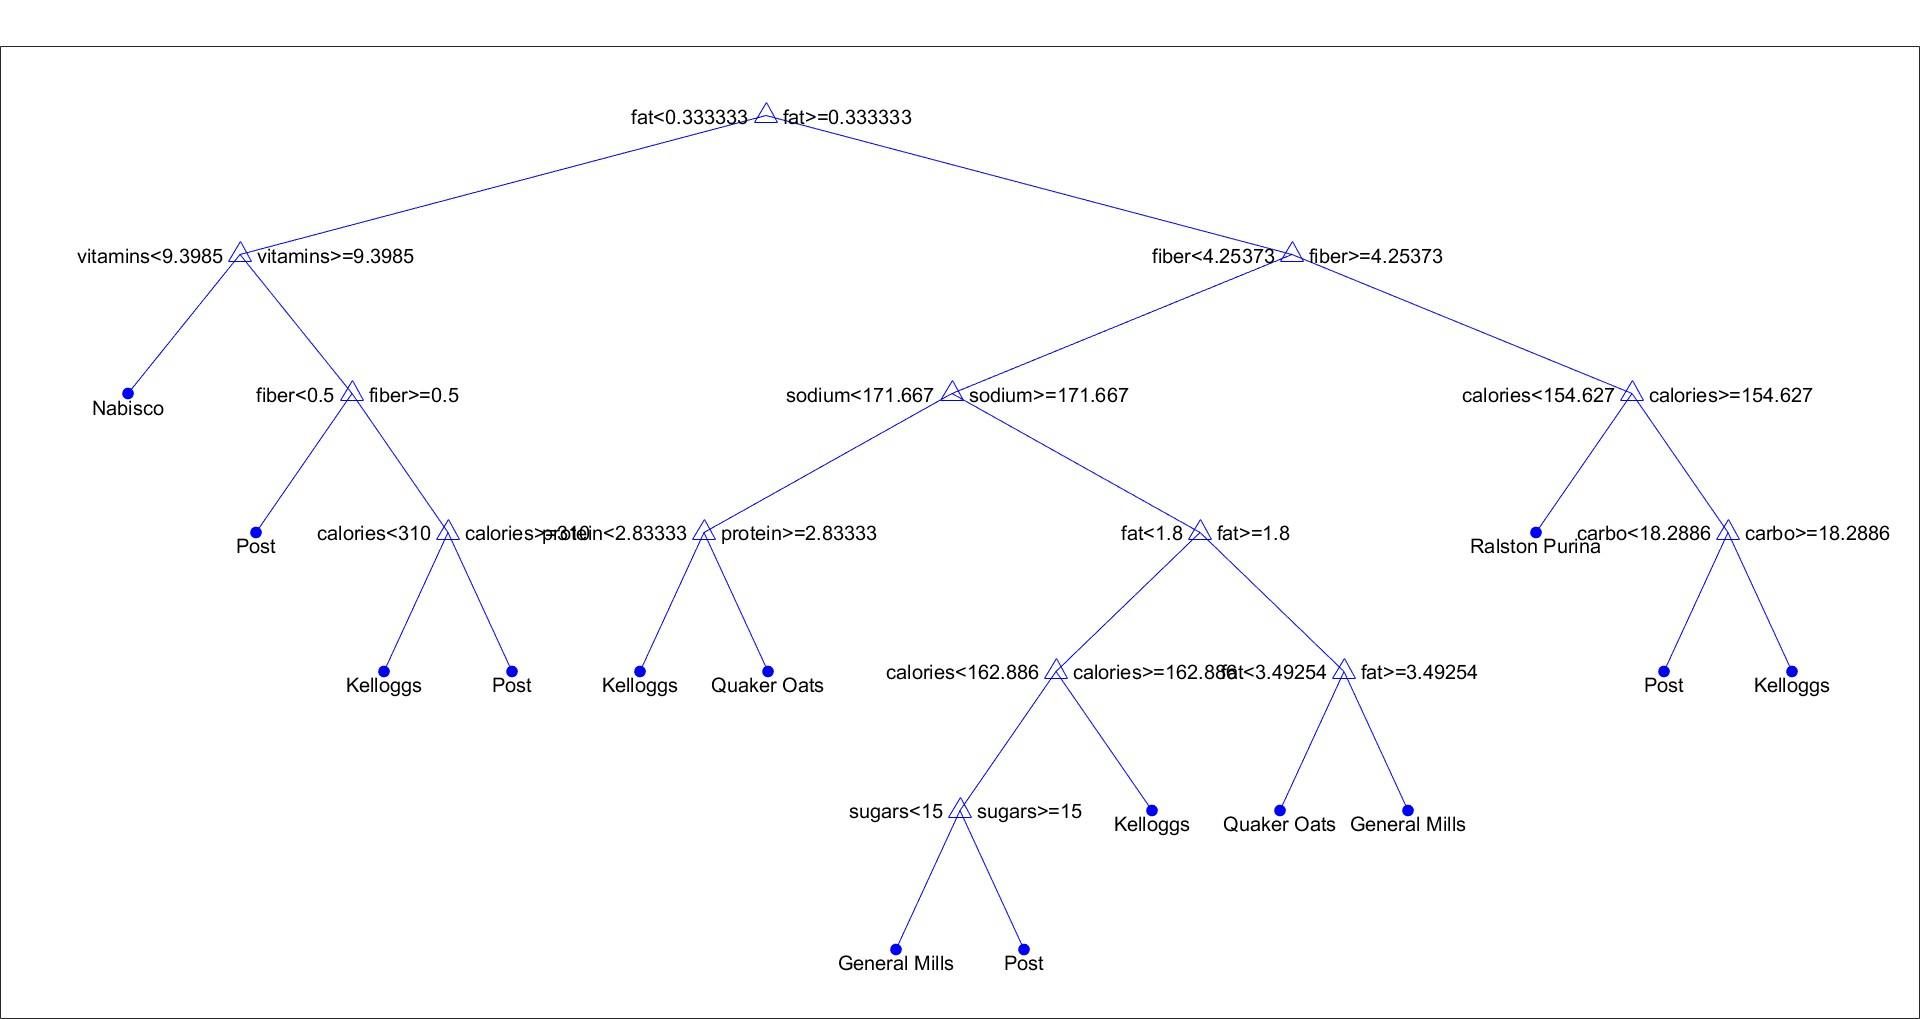
\includegraphics[width=\linewidth]{Cereal Tree Unpruned.jpg}
    \caption{Unpruned Tree}
    \label{fig:unpruned}
\end{figure}

\begin{figure}[tbp!]
    \centering
    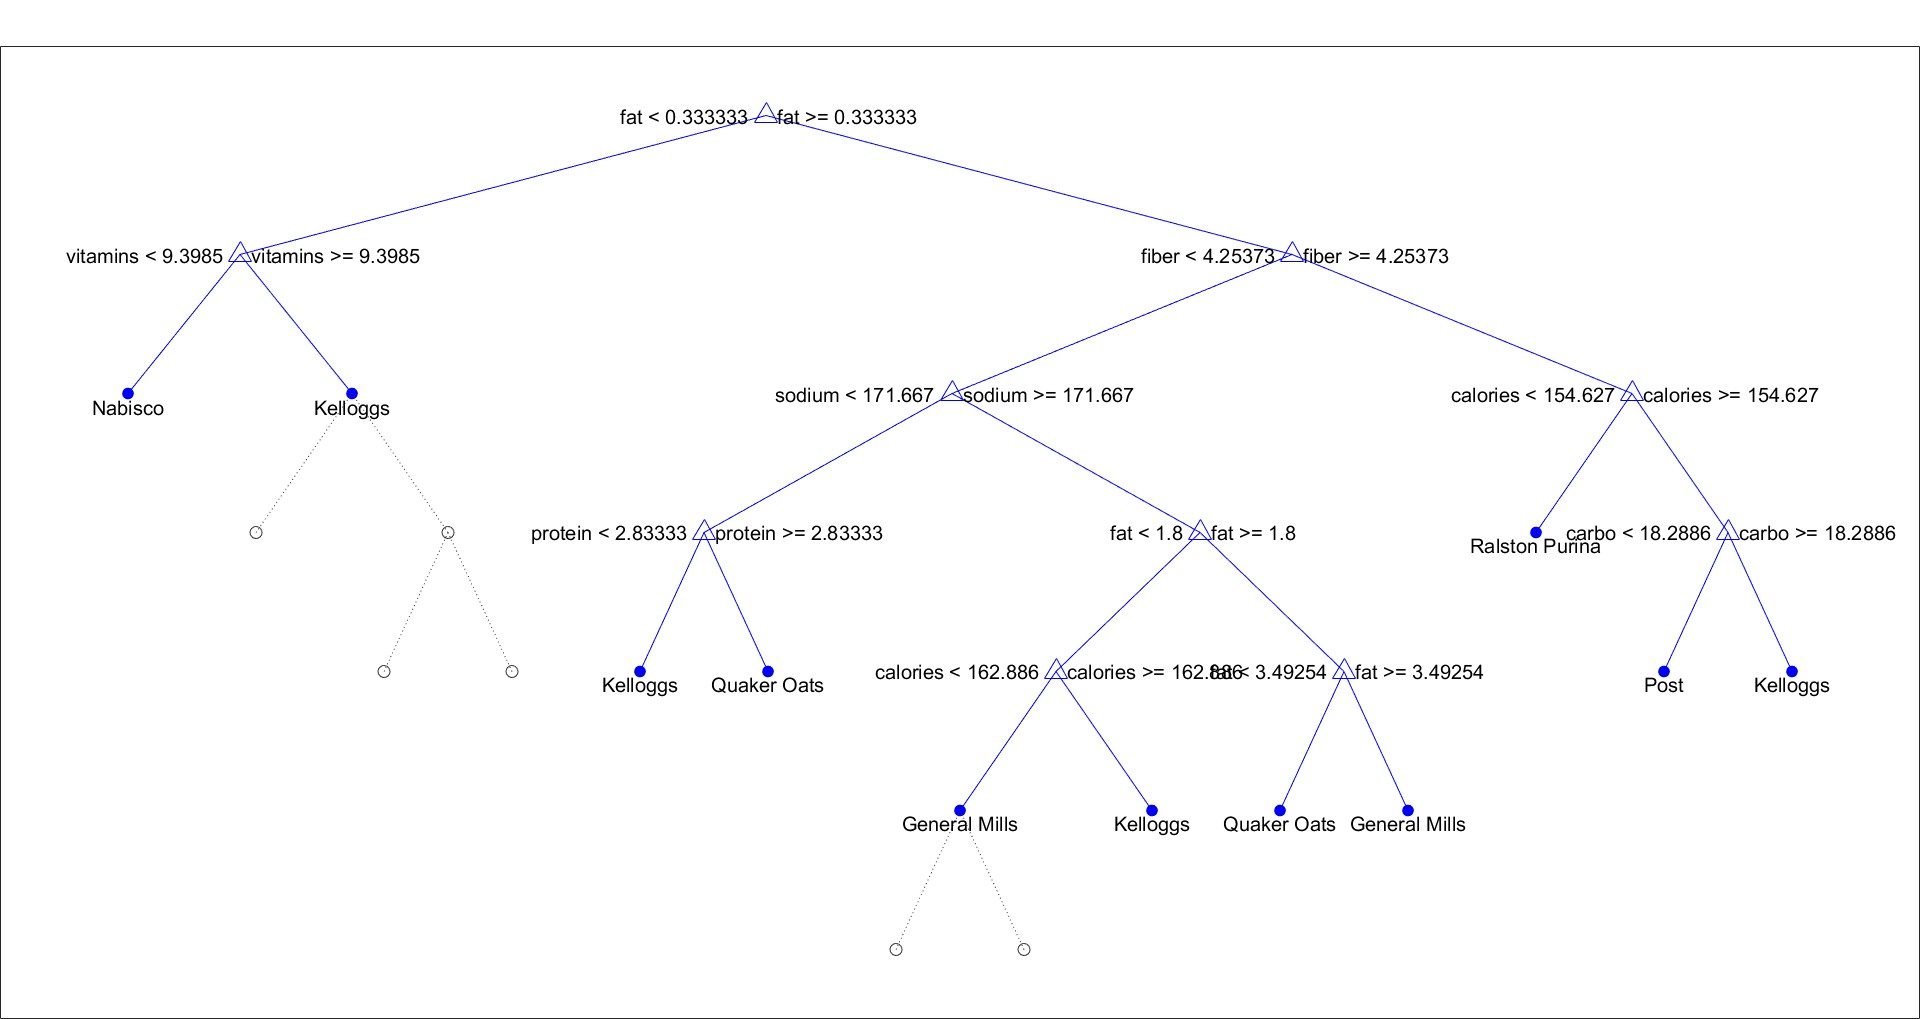
\includegraphics[width=\linewidth]{Cereal Tree Pruned 1.jpg}
    \caption{Tree Pruned Once}
    \label{fig:prune1}
\end{figure}

\begin{figure}[tbp!]
    \centering
    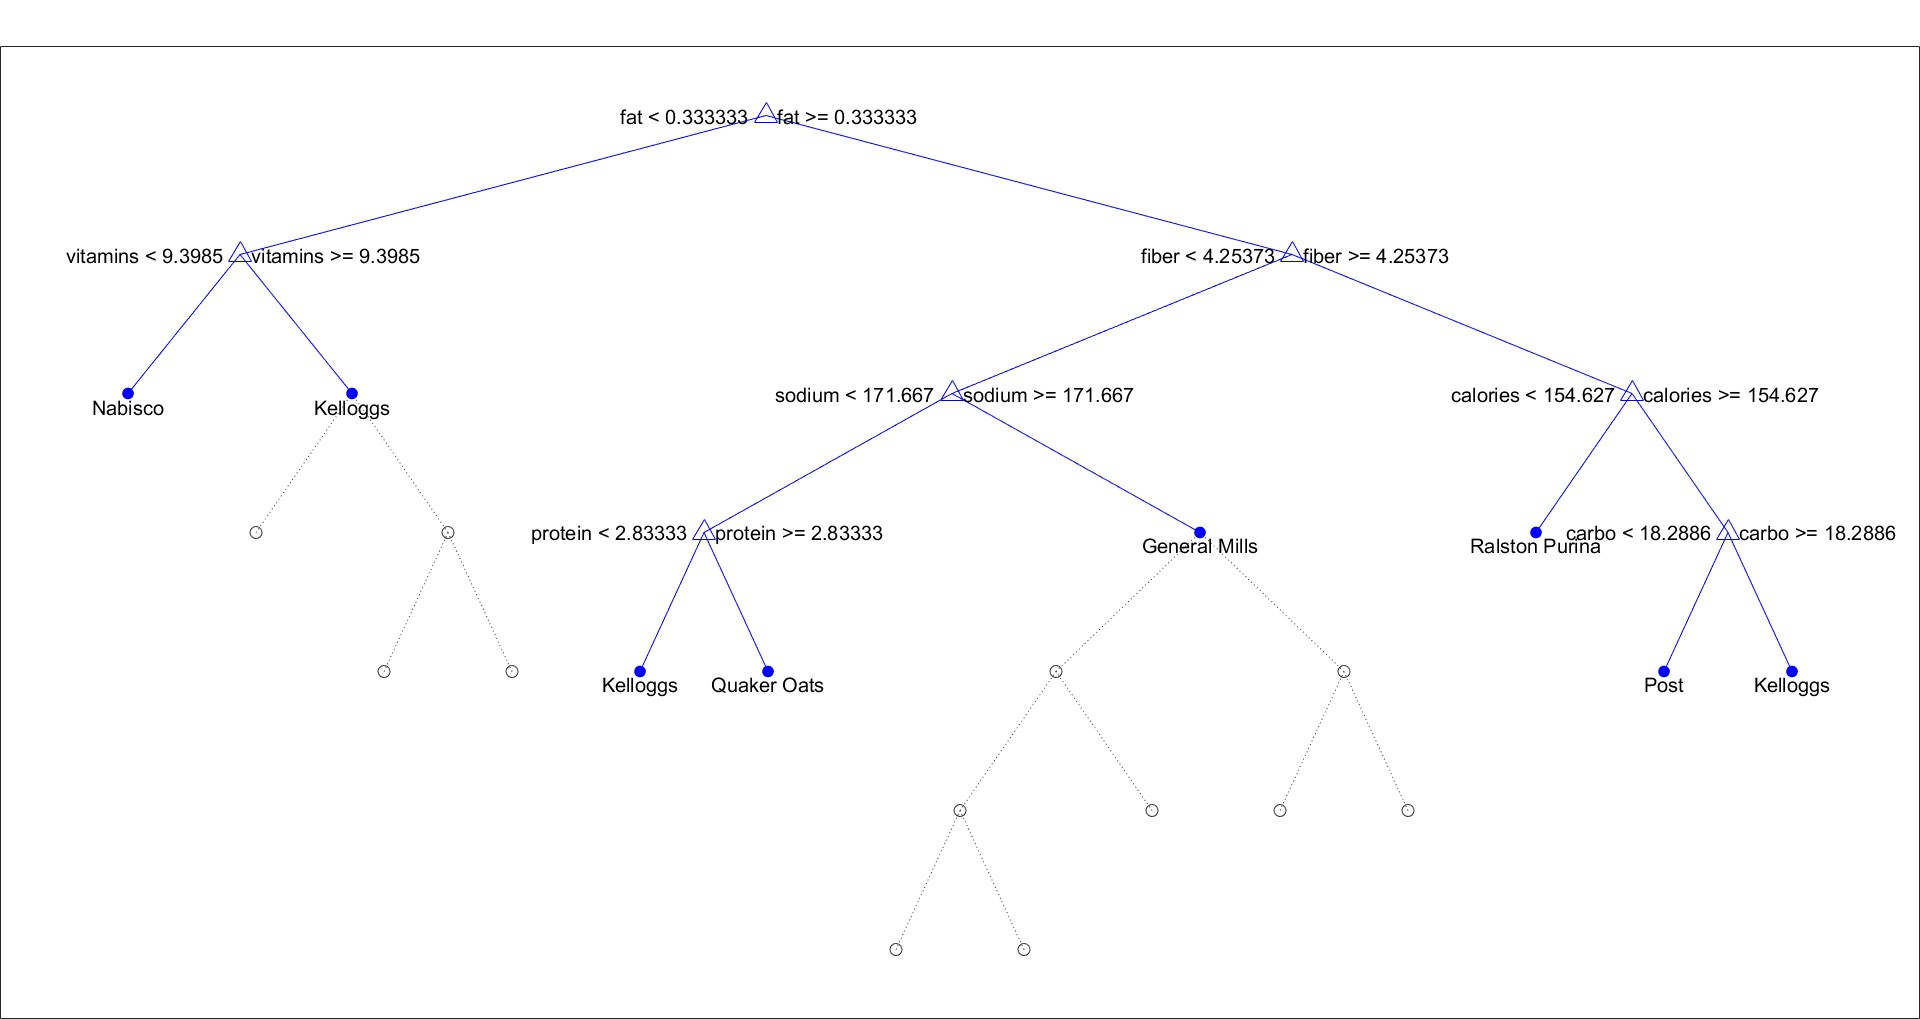
\includegraphics[width=\linewidth]{Cereal Tree Pruned 2.jpg}
    \caption{Tree Pruned Twice}
    \label{fig:prune2}
\end{figure}

\begin{figure}[tbp!]
    \centering
    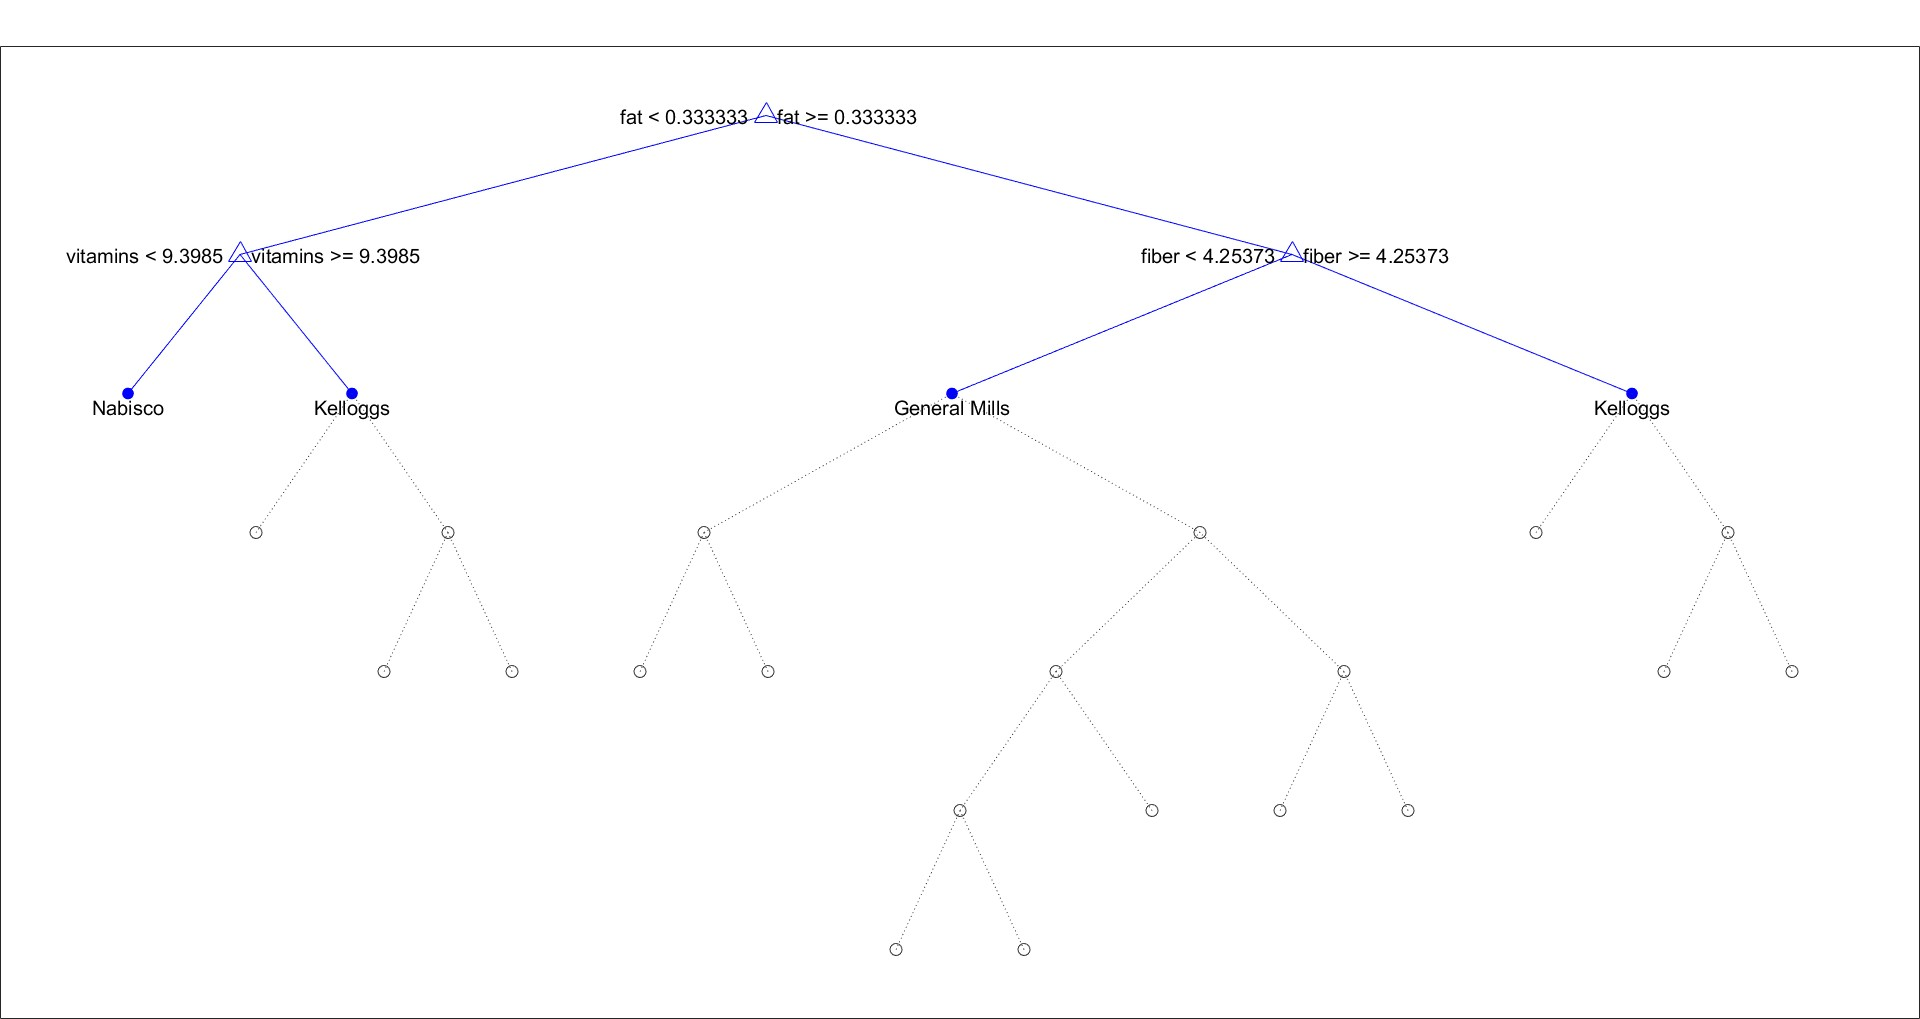
\includegraphics[width=\linewidth]{Cereal Tree Pruned 3.jpg}
    \caption{Tree Pruned Thrice}
    \label{fig:prune3}
\end{figure}

\begin{figure}[tbp!]
    \centering
    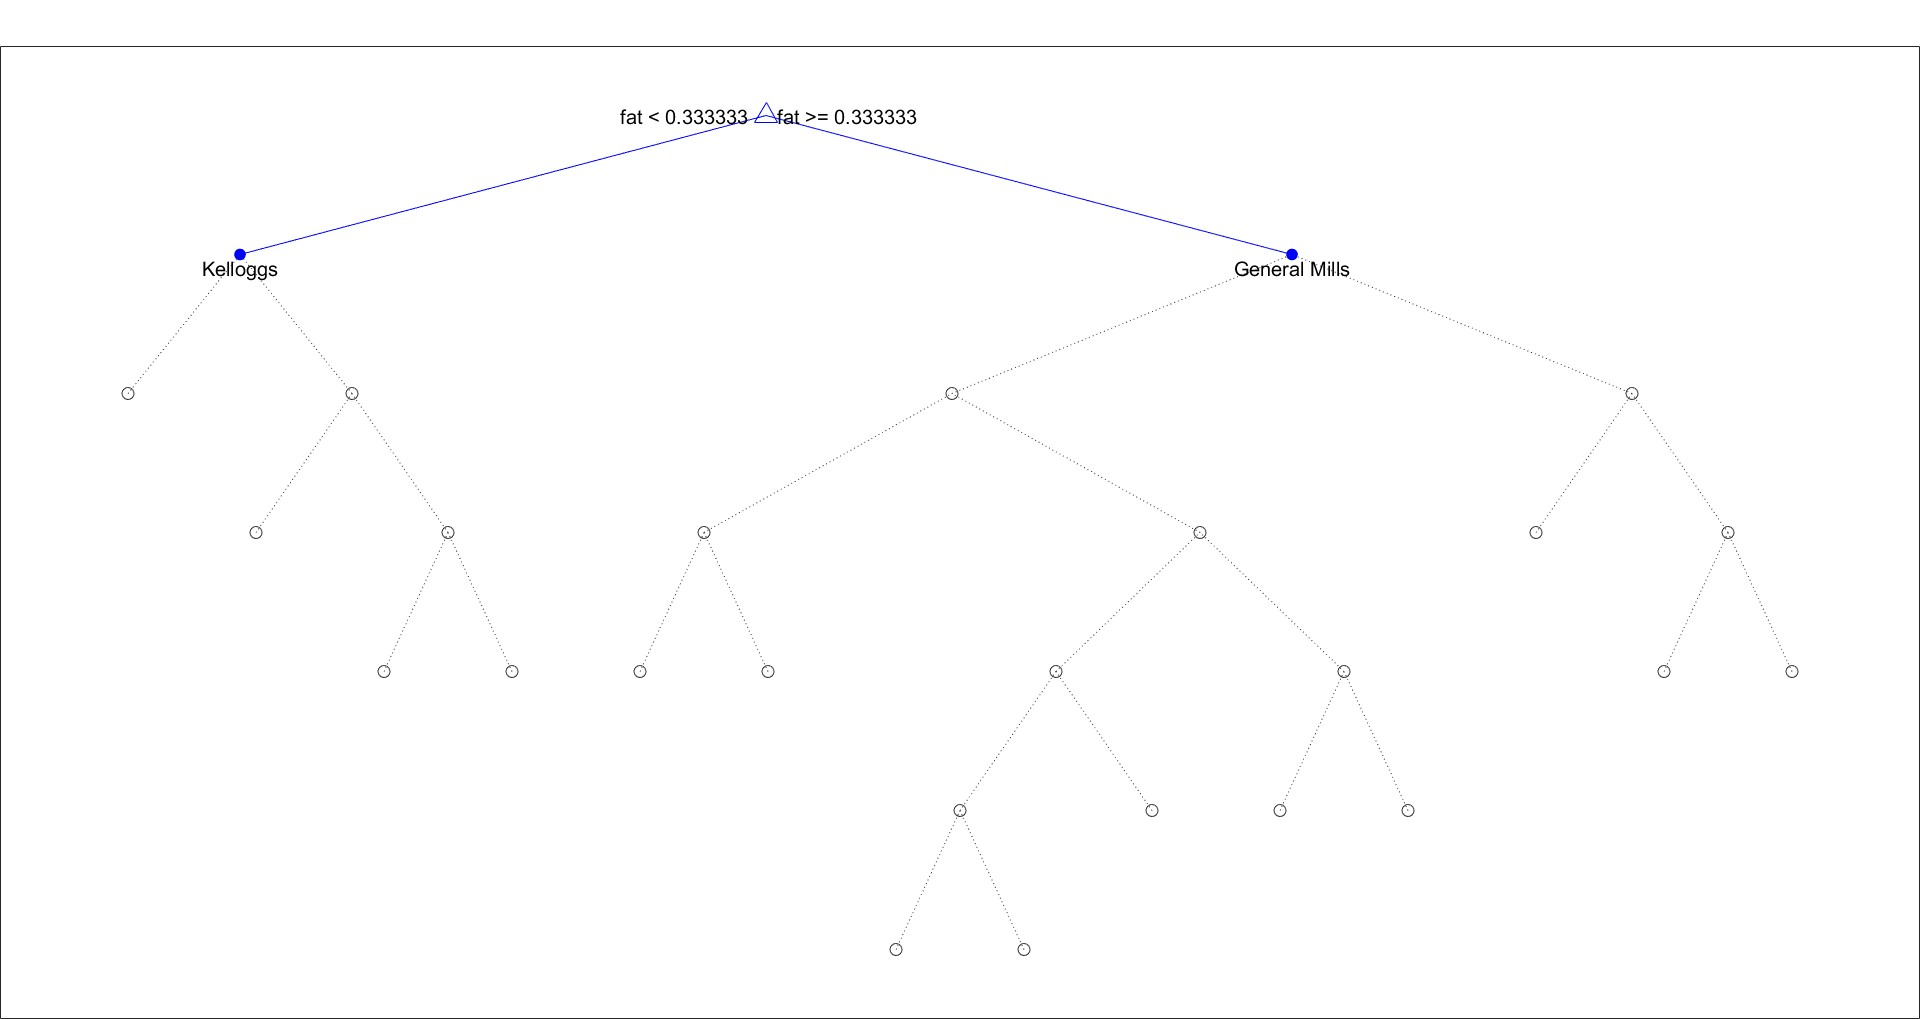
\includegraphics[width=\linewidth]{Cereal Tree Pruned 4.jpg}
    \caption{Maximally Pruned Tree}
    \label{fig:prune4}
\end{figure}

\section{Regression trees}

While classification and regression trees are quite similar, they vary in their exact applications. Classification trees only work on categorical dependent variables as discussed above, while regression trees can be used on continuous outputs and often yield stronger results due to their numerical nature. Instead of quantifying impurity in terms of Gini metric, misclassification rate, or some other metric, regression trees commonly use the mean squared error as the impurity metric, defined as
\[i(\tau)=\sum_{i=1}^n (y_i-y_{\text{mean}})^2\]
Impurity in regression trees is not defined to only exist between 0 and 1, and can easily reach into the millions with large trees. Because of this, it is much more difficult to directly compare node and tree impurity both within regression trees and with classification trees. Despite this, scaling the impurity of the terminal node with the total impurity of the tree can be done to determine the relative strength and contribution of each split. Often this contribution is given as
\[1-\frac{i(\tau)}{R(T)}\]
 with higher values corresponding to more significant contributions and lower values to less significant ones. \cite{zhang}

One notable trait of regression trees in particular is that they do not necessarily return a range of outcomes that spans the entire range of the training data, and this should be considered when analyzing their performance on both validation and practical data.

\section{Strengths and weaknesses of tree-based methods}

Just like any other method, CART has its own unique set of advantages and disadvantages. As a statistical method, CART is particularly robust when dealing with noisy or extraneous data. Because there should never be a single instance where an insignificant variable reduces impurity significantly, CART can altogether ignore it, as opposed to other methods that often will include it with low weighting.

CART is also very flexible with regard to data type and completeness. CART can handle numerical and categorical data simultaneously with ease, as all splits are binary and thus the same within the larger structure of the tree. It can similarly ignore missing data in large datasets in a way that a more traditional linear or logistic model cannot. This makes it useful when using real-world datasets that often have gaps.

The largest strength of CART, however, is its power in data visualization and interpretability. A tree is easily illustrated and can be understood by readers with absolutely no background in statistics, math, or data science. This makes it a superb way to explain the relationships in a digestible way that is basically unmatched by other methods.

While CART has these strengths, it is also important to consider its weaknesses. In comparison to other methods like logistic regression or neural networks, CART is quite fickle. CART is highly dependent on its training data, and changes to a single entry can completely change the structure of the tree produced. Similarly, CART is more prone to overfitting than many other methods; this is why pruning is so important, but data can still be overfit after pruning the tree as well. Because of these strengths, it is common for tree-based methods to be combined with other methods to create more robust algorithms, with random forests being one of the most notable examples of this.

By using CART in conjunction with other methods, one can easily develop a robust yet easily interpretable method for classifying cases and predicting outcomes. This is especially effective in medical settings, as previously stated, and academic ones \cite{breiman}, but can be applied to many other situations and datasets as well. As with any other method, as long as weaknesses are considered and accounted for, CART can be an exceptionally strong method of machine learning with broad applications.

\printbibliography[heading=bibintoc,title={Sources}]

\end{document}
